
\section{Circuit Example}
\label{sec:example}

\lstset{
  captionpos=b,
  language=Haskell,
  basicstyle=\scriptsize,
  numbers=left,
  numberstyle=\tiny,
  columns=fullflexible,
  stepnumber=1,
  escapechar=\#,
  keepspaces=true,
  literate={<}{{$\langle$}}1 {>}{{$\rangle$}}1,
  morekeywords={function,rr,int,float,bool,isnull,partition,as,downregion,upregion,reads,writes,rdwrs,reduces,read,write,reduce,using,unpack,pack,coloring,multicoloring,color,newcolor,atomic,simultaneous},
  deletekeywords={head,min,max}
}

We begin by introducing an example program 
motivating the novel features of Legion.
Due to space constraints we present only code fragments;
the full example is in the submitted appendix.

Consider a simulation of an electrical circuit.
The simulation runs for many time steps, each of which performs three computations:
 calculate new currents, distribute charges, and update voltages.
The simulation takes as input an arbitrary graph of circuit elements
that have been dynamically allocated in two logical regions: {\tt all\_nodes} 
and {\tt all\_wires}.  The types of nodes and wires are 
shown in Listing~\ref{lst:tuples}.  The first two fields in the
{\tt CircuitWire} tuple are pointers that specify the two end points of
a wire.  Pointers are denoted by the @ symbol
followed by the region(s) into which the pointer may point.
The {\tt CircuitWire} type is parametrized by the local region
names {\tt rn} and {\tt rg} which contain {\tt CircuitNode} elements.
Our type system enforces the correctness of pointer types.

\begin{lstlisting}[label={lst:tuples},caption={Tuples and Pointers Example}]
--                        voltage,current,charge,capacitance,piece ID
type CircuitNode        = <float,float,float,float,int>
--                      owned node, owned or ghost node, resistance, current
type CircuitWire<rn,rg>  = <CircuitNode@rn, CircuitNode@(rn,rg),float,float>
\end{lstlisting}

The most important decision in any Legion program is how to partition
program data.  An ideal partitioning depends on many factors,
including the shape of data structures, the input, and the number of
partitions, which usually varies with the target machine.  To allow
the necessary flexibility, in Legion partitioning is simply programmed,
rather than expressed in a more structured and restricted
sublanguage.  In the example we invoke METIS\cite{Metis98}, a 
third-party dynamic graph partitioning library (see Listing~\ref{lst:metis}).

\begin{lstlisting}[label={lst:metis},caption={Partition Computation}]
type NodeList<rl,rn>       = < CircuitNode@rn, NodeList<rl,rn>@rl >
type WireList<rl,rw,rn,rg>= < CircuitWire<rn,rg>@rw, WireList<rl,rw,rn,rg>@rl >
function extern_metis[rl,rn,rw](node_list : NodeList<rl,rn>@rl,
          wires_list : WireList<rl,rw,rn,rn>@rl), reads(rl,rn,rw), writes(rn) : bool
\end{lstlisting}

METIS takes as arguments lists of the nodes and wires in
the graph.  It breaks the graph into pieces by annotating each 
{\tt CircuitNode} with a piece ID (the last field of the tuple).
The function {\tt extern\_metis} is parametrized on the regions it 
accesses: {\tt rn} is a region of nodes, {\tt rw} is a region of wires, 
and {\tt rl} is a region with the lists of pointers.  The function
also specifies the access {\em privileges} (e.g read, write) it requires for each 
region.  All three regions are read by {\tt extern\_metis}, but only the {\tt rn}
region is written (since it writes the piece ID).  A function can only 
have privileges that its caller also possesses; this property is verified statically. 
% by the Legion type system.

\begin{figure}[t]
\centering
\subfigure[Node region tree.]{
\label{sfig:part_fig:tree}
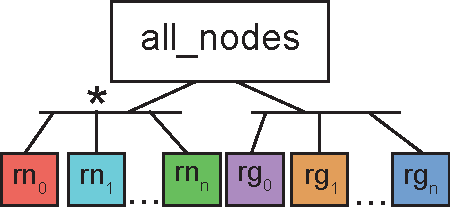
\includegraphics[scale=0.50]{figs/OwnedTree.pdf}
}
\subfigure[Circuit piece coloring.]{
\label{sfig:part_fig:pieces}
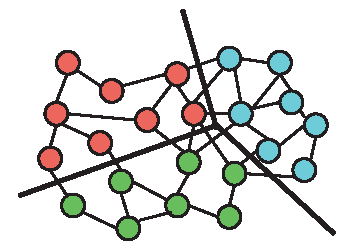
\includegraphics[scale=0.67]{figs/Owned_Nodes.pdf}
}
\subfigure[Ghost {\tt rg0} coloring.]{
\label{sfig:part_fig:ghost_zero}
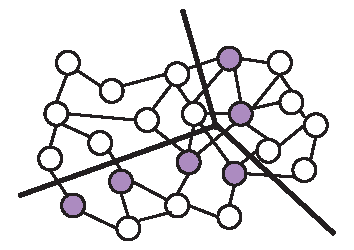
\includegraphics[scale=0.67]{figs/Ghost_RN0.pdf}
}
\subfigure[Ghost {\tt rg1} coloring.]{
\label{sfig:part_fig:ghost_one}
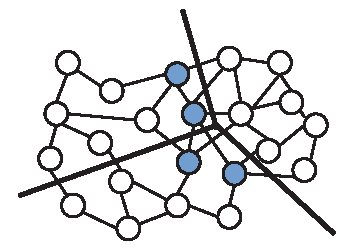
\includegraphics[scale=0.67]{figs/Ghost_RN1.pdf}
}
\vspace{-2mm} 
\caption{Partitions of $r{\_}all{\_}nodes$. \label{fig:part_fig}}
\vspace{-6mm}
%  \caption[My caption
\end{figure}

To efficiently support the access patterns of the circuit simulation,
the {\tt all\_nodes} region is partitioned in two different ways.  The
desired {\em region tree} is shown in Figure~\ref{sfig:part_fig:tree}.
First, there are {\em subregions} of {\tt all\_nodes} that describe
the set of nodes ``owned'' by each piece, called {\tt rn0}, {\tt rn1},
$\ldots$. Since each node is in one piece, this partition is {\em
disjoint} (indicated by a $*$ on the left subtree).
Figure~\ref{sfig:part_fig:pieces} shows one possible node partition;
different colors identify different piece IDs.  Second, each piece of
the circuit needs access to the nodes on its border, commonly referred
to as {\em ghost nodes}.  The ghost nodes for two circuit pieces are
shown in Figures~\ref{sfig:part_fig:ghost_zero}
and~\ref{sfig:part_fig:ghost_one}; note two nodes are in both sets.
Because a node may neighbor more than one other circuit piece, this
second partition of {\tt all\_nodes} is {\em aliased}.  Thus, there
are two sources of aliasing in the region tree: the two distinct partitions
divide the {\tt all\_nodes} region in different ways, and the ghost
node subregions are not disjoint.

Note there are two alternative approaches to using multiple partitions,
both of which avoid introducing aliasing:
first, we could create a single partition with $2^n$ subregions, one for each
possible case of sharing; second, tasks for each piece could use the
{\tt all\_nodes} region to access their ghost nodes.  Neither option
is attractive: the former significantly complicates programming, the
latter greatly increases runtime data movement and would limit parallelism.

Programmers express partitions using {\em colorings},
maps from region elements to integers (``colors'').
Listing~\ref{lst:coloring} shows the function {\tt create\_piece\_coloring}
that constructs a coloring from the piece IDs of a list of nodes.
%The coloring of wires is similar, with each wire
%using the color of its first endpoint.  
For aliased partitions such as the ghost nodes, a {\em multicoloring}
is used, which assigns each region element to one or more colors.  
%(Multicolorings are
%implemented in Core Legion with separate colorings for each color.)
\begin{lstlisting}[label={lst:coloring},caption={Coloring Construction}]
function create_piece_coloring[rl,rn](node_list: NodeList<rl,rn>@rl),
            reads(rl,rn) : coloring(rn) = 
    if isnull(node_list) then
        newcolor(rn) 
    else                                 -- tuple fields accessed by .(field number)
        let list_elem : NodeList<rl,rn> = read(node_list) in
        let part_coloring : coloring(rn) = create_node_coloring(list_elem.2) in
        let node : CircuitNode = read(list_elem.1) in
            color(part_coloring, list_elem.1, node.5)
\end{lstlisting}

Colorings are the input to partition operations in Legion.  The partition
statement shown in Listing~\ref{lst:partition} performs the ``owned nodes''
partitioning.    Since colorings assign each region element at most one color
(dynamically checked), the partition operation results in 
{\em disjoint} subregions, each a subset of the {\em parent} region.
A partition operation introduces constraints into the static type environment describing
both the disjointness of subregions (e.g., {\tt rn0 $*$ rn1})
and the subregion relationships
(e.g., {\tt rn0 $\leq$ all\_nodes}).  A partition created from a multicoloring
only introduces the subregion relationships, as the partition may be aliased.



%The partitioning of wires is identical, while the partitioning
%of the ghost nodes is performed in Core Legion as a separate partitioning operation
%for each color.

\begin{lstlisting}[label={lst:partition},caption={Partition Operation Example}]
let piece_coloring : coloring(all_nodes) = create_piece_coloring[rl,all_nodes](node_list) in
partition all_nodes using piece_coloring as rn0,rn1... in ...
\end{lstlisting}


%% In addition, to partitioning the graph to describe {\em owned} nodes
%% for each piece, the circuit example also
%% needs to be able to name the {\em ghost nodes} for each piece.  Ghost node
%% regions are used for accessing the nodes of wires that span
%% two different pieces. (This is also the reason {\tt CircuitWire} is parametrized on
%% two regions).  Figure~\ref{sfig:part_fig:ghost_zero} and 
%% Figure~\ref{sfig:part_fig:ghost_one} show colorings for the ghost regions
%% corresponding to {\tt rn0} and {\tt rn1} respectively.  Note that two 
%% nodes are colored in both colorings.  Since nodes can appear in multiple
%% subregions, we use a {\em multicoloring} (implemented in core Legion
%% by multiple single colorings) to describe {\em aliased} partitions.  Aliased
%% partitions still introduce subregion constraints into the static checking
%% environment, but not disjointness constraints.  Figure~\ref{sfig:part_fig:tree}
%% shows the resulting logical region tree for node regions.

The first-class nature of logical regions in Legion allows them to
be written into the heap.  To avoid losing information about these regions and pointers
into those regions, Legion provides {\em region
relationships}.  Region relationships are a bounded existential type
that allows programmers to {\em pack} a group of regions and pointers together and capture
properties about them such as disjointness and subregion relationships.
Listing~\ref{lst:rr} shows an example region relationship for a {\tt CircuitPiece} 
describing its region of wires {\tt rpw}, region of 
nodes {\tt rpn}, region of ghost nodes {\tt rg}, and important constraints.  Although the
``names'' of {\tt rpw}, {\tt rpn}, and {\tt rg} are lost when packed into the region relationship,
the knowledge that they are subregions of the {\tt rw} and {\tt rn} regions is not.

\begin{lstlisting}[label={lst:rr},caption={Region Relationship Example}]
type CircuitPiece<rl,rw,rn> = rr[rpw,rpn,rg]  -- rr is keyword for region relationship 
                            < WireList<rl,rpw,rpn,rg>@rl, NodeList<rl,rpn>@rl >         
                            where rpn #$\le$# rn and rg #$\le$# rn and rpw #$\le$# rw and
                                  rn * rw and rl * rn and rl * rw
\end{lstlisting}

The Legion type system verifies properties of region relationships when packing.  When
a region relationship is unpacked later, fresh names are given to the regions that were
captured by the region relationship (passed in {\tt []} parameters), and the properties that are known to hold for these
regions are re-introduced to the type environment.
In contrast, region access privileges cannot be packed in a region
relationship---privileges belong to functions. When a function unpacks
a region relationship it must already hold privileges for the unpacked regions it wishes to access.

Listing~\ref{lst:loop} shows the main time step loop run by the 
recursive function {\em execute\_time\_steps} (line 11)
as well the leaf task functions (lines 2-7).  
For each time step, the loop unpacks 
two previously packed circuit pieces, giving new names to the subregions introduced
by each region relationship.  The {\em execute\_time\_steps} function
will have read/write privileges for the newly named regions, such as {\tt rn0},
because it has read/write privileges for {\tt rn} and the {\tt CircuitPiece} 
region relationship ensures that {\tt rn0 $\leq$ rn}.

The {\tt execute\_time\_steps} function   
illustrates the importance of having different partitions provide 
multiple views onto the same logical region.  Both {\tt calc\_new\_currents} 
and {\tt distribute\_charge} (lines 2-5)
use the owned and ghost regions of a piece, which are from different partitions. In
{\tt calc\_new\_currents} these regions only need read
privileges, allowing both instances of the task to be
run in parallel.  In {\tt distribute\_charge} the
privilege is for a reduction which can also be done in parallel
because of the atomic and commutative nature of reductions.  Finally,
the {\tt update\_voltage} function (line 6) modifies only the disjoint owned regions, 
permitting each piece to be updated in parallel.  No single partition of the nodes
describes these data sharing patterns.

\lstset{
  captionpos=b,
  language=Haskell,
  basicstyle=\scriptsize,
  numbers=left,
  numberstyle=\tiny,
  columns=fullflexible,
  stepnumber=1,
  escapechar=\#,
  keepspaces=true,
  belowskip=-10pt,
  literate={<}{{$\langle$}}1 {>}{{$\rangle$}}1,
  morekeywords={function,rr,int,float,bool,isnull,partition,as,downregion,upregion,reads,writes,rdwrs,reduces,read,write,reduce,using,unpack,pack,coloring,multicoloring,color,newcolor,atomic,simultaneous},
  deletekeywords={head,min,max}
}
\begin{lstlisting}[float={t},label={lst:loop},caption={Main Simulation Loop}]
-- Leaf Task Declarations (implementations in appendix)
function calc_new_currents[rl,rw,rn,rg] ( ptr_list : WireList<rl,rw,rn,rg>@rl ), 
      reads(rl,rw,rn,rg), writes(rw) : bool
function distribute_charge[rl,rw,rn,rg] ( ptr_list : WireList<rl,rw,rn,rg>@rl ), 
      reads(rl,rw,rn), reduces(reduce_charge,rn,rg), atomic(rn,rg) : bool 
function update_voltage[rl,rn] ( ptr_list : NodeList<rl,rn>@rl ), 
      reads(rl,rn), writes(rn) : bool
-- Reduction function for distribute charge
function reduce_charge ( node : CircuitNode, current : float ) : CircuitNode

-- Time Step Loop
function execute_time_steps[rl,rw,rn] ( p0 : CircuitPiece<rl,rw,rn>, 
      p1 : CircuitPiece<rl,rw,rn>, steps : int ) , reads(rn,rw,rl), writes(rn,rw) : bool = 
  if steps #$<$# 1 then true else
  unpack p0 as piece0 : CircuitPiece<rl,rw,rn>[rw0,rn0,rg0] in 
  unpack p1 as piece1 : CircuitPiece<rl,rw,rn>[rw1,rn1,rg1] in
  let _ : bool = calc_new_currents[rl,rw0,rn0,rg0](piece0.1) in
  let _ : bool = calc_new_currents[rl,rw1,rn1,rg1](piece1.1) in
  let _ : bool = distribute_charge[rl,rw0,rn0,rg0](piece0.1) in
  let _ : bool = distribute_charge[rl,rw1,rn1,rg1](piece1.1) in
  let _ : bool = update_voltage[rl,rn0](piece0.2) in
  let _ : bool = update_voltage[rl,rn1](piece1.2) in
      execute_time_steps[rl,rw,rn](p0,p1,steps-1)
\end{lstlisting}

The {\tt execute\_time\_steps} function also demonstrates the need to 
dynamically discover parallelism through region disjointess.  
To run the two instances of 
{\tt calc\_new\_currents} in parallel requires knowing that {\tt rw0}
and {\tt rw1} are disjoint (lines 17-18).  There is a similar requirement for parallel
execution of the two {\tt update\_voltage} calls with {\tt rn0} and {\tt rn1} (lines 21-22).  In
both cases, this knowledge was statically available when the subregions were created 
and could have been captured in a region relationship at the cost
of much more complicated code.  Instead, we use a simpler region relationship
and rely on an inexpensive dynamic disjointness
check by the Legion runtime to (re)discover the parallelism.

In addition to privileges, functions can also specify {\em coherence}
on regions.  By default, coherence on all regions is {\em exclusive}, meaning
the function must appear to execute in program order relative to other function
calls that access non-disjoint data.  Programmers can allow other
execution orderings using relaxed coherence.  Line 5 of Listing~\ref{lst:loop} shows
an example of {\tt atomic}, a relaxed coherence mode requiring
that operations to {\tt rn} and {\tt rg} appear atomic relative
to other functions using regions which may alias.  The most relaxed coherence
mode is {\tt simult}; simultaneous coherence allows concurrent access 
to the region by all functions that are using the region
in a simultaneous mode.  The interaction between {\em tasks} (which are functions 
chosen to execute in parallel) using the same region with different coherence
modes is formalized in Section~\ref{sec:coherence}.

%The most important decision in any Legion program is the choice of
%how to partition program data into logical regions.  Logical regions
%are the granularity at which the Legion runtime will reason
%about the independence of tasks, and therefore how much parallelism
%is available.  Logical regions also define the granularity at which
%the Legion runtime will move data.  Coarser regions will lead
%to more efficient bulk copies of data throgh the memory hierarchy due
%to better locality.  There is therefore a natural tension: partitioning 
%should be fine-grained enough to express desired parallelism, but not 
%so fine-grained as to result in inefficient data movement.

%The first step in the circuit example is to partition the arbitrary graph
%of circuit elements into pieces that can be handled independently.
%In the case of this example all nodes in the graph have initially
%been allocated in the region {\tt all\_nodes} (Figure~\label{sfig:part_fig:tree}).
%The decision of how to partition the graph is the responsibility
%of the programmer and can be done by an external library (e.g. METIS
%in this case).  Once the decision of how to partition is made, the
%result must be communicated to the Legion runtime to 
%generate the corresponding logical regions.  Partitioning decisions
%are described via {\em colorings}.  Colorings are parametrized by
%the region they are partitioning and capture a mapping from pointers
%into the region to specific colors (e.g. integers).  Figure~\ref{sfig:part_fig:pvs}
%illustrates the coloring used for generating the {\tt p\_nodes\_pvs}
%partition.



